\subsection{Stochastic Games}
We consider a graph-based game formalism between two players. A
(2.5-player) \emph{stochastic game} (SG) is a tuple $\sg = \langle S,
\iota, \Act, P \rangle$.  The set of \emph{states} $S = S_\pOne \cup
S_\pTwo$ is partitioned into a set $S_\pOne$ of (controlled)
$\pOne$-states and a set $S_\pTwo$ of (uncontrolled)
$\pTwo$-states. $\iota \in S_\pTwo$ is the \emph{initial state}, $\Act$ is a
finite set of \emph{actions}, and $P\colon S \times \Act \rightarrow
\Distr(S)$ is the \emph{transition function}. For simplicity of
exposition, we shall assume w.l.o.g. that controlled and uncontrolled
states alternate. Thus, $P$ is defined by two partial transition functions:
$P_\pOne\colon S_\pOne \times \Act \rightarrow \Distr(S_\pTwo)$,
$P_\pTwo\colon S_\pTwo \times \Act \rightarrow \Distr(S_\pOne)$. We
identify the available actions\footnote{We explicitly allow to model
unavailable actions, e.g., we can model that a door can only opened
when close enough to the door.} as $\EnAct(s) \eqdef \{ \act \mid
P(s,\act) \neq \bot \}$. States without available actions, i.e.,
states with $\EnAct(s) = \emptyset$ are called \emph{terminal states}.
A SG is finite, if its state space is finite.  The \emph{successor
states} of a state $s$ and an (enabled) action $\act$ is the set of
states that are reached from $s$ within one step with a positive
transition probability, i.e., $\Succ(s,\act) \eqdef \{ s' \mid
P(s,\act)(s')>0 \}$, and $\Succ(s) \eqdef\bigcup_{\act \in \EnAct(s)}
\Succ(s,\act)$.


\begin{figure}
\centering
\begin{tikzpicture}
	\node[sstate] (s0) {$s_0$};
	\node[astate,right=of s0] (s1) {$s_1$};
	\node[sstate,below=of s1] (s2) {$s_2$};
	
	\node[tstate,right=1.4cm of s1] (target) {$\target$};
	\node[tstate,right=1.4cm of s2] (sink) {$\sink$};
	
	\node[actnode,right=4mm of s1] (a1) {};
	\node[actnode,right=4mm of s2] (a2a) {};
	
	
	\draw[->] (s0) -- node[actnode] {} 
	                  node[near start,auto,elab] {$a$} (s1);
	\draw[->] (s0) -- node[actnode] {}
					  node[near start,elab,below] {$b$} (s2);
	\draw[->] (s1) -- node[actnode] {}
					  node[near start,elab] {$b$}  (s2);
	\draw[->] (s1) -- node[elab] {$a$} (a1);
	\draw[->] (a1) -- node[elab] {$\nicefrac{1}{3}$} (target);
	\draw[->] (a1) -- node[elab,near start] {$\nicefrac{2}{3}$} (sink);
	\draw[->] (a2a) -- node[elab] {$\nicefrac{1}{3}$} (target);
	\draw[->] (a2a) -- node[elab,near start] {$\nicefrac{2}{3}$} (sink);
	\draw[->] (s2) -- node[elab] {$a$} (a2a);
	\draw[->] (s2) edge[bend right=30] node[actnode] {}
										node[near start,below] {$b$} (sink);
	
	
\end{tikzpicture}	
\caption{A running example. }
\label{fig:toysg}
\end{figure}
\begin{example}
  We introduce a 5 state toy-example~(Fig.~\ref{fig:toysg}) to
  illustrate the formalisms. Terminal states are drawn with a rectangle,
  $\pOne$-states with a circle and $\pTwo$-states with a diamond. For
  every state $s$ and action $\act$, we draw transitions in the form
  of edges that connect all successors $s'$, and label them with the
  associated probaiblities $P(s,\act)(s')$. For conciseness, we omit
  labelling probability $1$ transitions.
\end{example}
	

SGs capture a variety of models.  For example, if $\Act_\pOne$ is a
singleton set, then $\sg$ is a \emph{Markov decision process} (MDP).
If both $\Act_\pOne$ and $\Act_\pTwo$ are singleton sets, then $\sg$ is a
\emph{Markov chain}. If $P(s,\act)$ is a Dirac distribution for every
$s \in S$ and $\act \in \Act$, then $\sg$ is called
\emph{deterministic} or a \emph{2-player game}.

\subsection{Paths and Path Properties}
A finite \emph{path}, $\path$, of length $n$ is a sequence $s^0
\xrightarrow{\act_0} s_1 \xrightarrow{\act_1} s_2 \rightarrow \hdots
\rightarrow s_n$ in $\left( S \times \Act \right)^{n} \times S$ where
$P(s_i,\act_i)(s_{i+1}) > 0$ for each $i$.  We denote the length with
$|\path|$, and denote $s_n$, i.e., the last element of $\path$ with
$\last{\path}$. Further, note that $\pTwo$ states are even
indexed and $\pOne$ states are odd indexed by our ordering
assumption.
A path, $\path' = s'_0 \xrightarrow{\act'_0} \hdots$, is a
\emph{prefix} of $\path$, if for all $i \leq |\path'|$, $s_i = s'_i$
and for all $i < |\path'|$, $\act_i = \act'_i$.  The set of all finite
paths of length $n$ is denoted $\Paths[n]{\sg}$, and $\Paths{\sg} =
\bigcup_{n \in \NN} \Paths[n]{\sg}$. We omit $\sg$ whenever it is
irrelevant or clear from the context.
It is helpful to partition paths
based on their last state: $\POnePaths[]{} = \{ \path \in
 \Paths[]{} \mid \last{\path} \in S_\pOne \}$ and $\PTwoPaths[]{} =
\Paths[]{} \setminus \POnePaths[]{}$.



\begin{example}
  In Fig.~\ref{fig:toysg}, there are two paths that end in $s_2$, $s_0 \xrightarrow{a} s_1 \xrightarrow{b} s_2$ of length $2$ and $s_0 \xrightarrow{b} s_2$ of length $1$. Both paths are in $\PTwoPaths[]{}$.
\end{example}
%\paragraph{Policies.} 
Whenever some state $s$ is reached, the corresponding player draws an action from $\EnAct(s)$. As standard, we capture this with the notion of a scheduler\footnote{Also known as \emph{strategy} or \emph{policy}.}.
A \emph{scheduler} is a tuple of \emph{player policies} $\sched = \langle \sched_\pOne, \sched_\pTwo \rangle$
with $\sched_{\player} \colon \PlayerPaths[]{} \rightarrow \Distr(\Act)$ such that $\supp(\sched_i(\path)) \subseteq \EnAct(\last{\path})$ for each $\path$, i.e., for every history, the policy sets a distribution over the enabled successor actions.
We will denote by $\sched_{\player}(\act~|~\path)$ the distribution of actions given the path, $\path$, induced by policy $\sched_{\player}$.
%We refer to $\sched_i$, $i \in \{ 1, 2 \}$ as a \emph{Player-i policy}. 
%We denote the $\pOne$-policy $\pOneSched$ and the $\pTwo$-policy $\pTwoSched$ with $\sched_\pOne$ and $\sched_\pTwo$, respectively.
To ease notation, we liberally use the notation $\sched \colon \Paths{} \rightarrow \Distr(\Act)$ where this function is given dependent on which player owns the last state.
 
%
%Applying a policy $\sched$ to an SG $\sg$ yields an \emph{induced Markov chain} $\induced{\sg}{\sched} = \langle S', \iota', P' \rangle$ with state space $S' = \Paths{\sg}$, initial state $\iota' = \iota$, and transition function $P'(\path,\path')$ defined by $P'(\path)(\path \cdot \act s') = \sched(\path)(\act) \cdot P(\last{\path},\act)(s')$ and $P'(\path,\path') = 0$ otherwise. For any upper bound on the length of the paths, the induced MC is finite. 


\begin{example}
  An example for a $\pOne$-policy $\pOneSched$ is given
  by,
  \begin{equation}
    \pOneSched(\alpha~|~\xi) =
    \begin{cases}
      1 & \text{if } \alpha = a,~\xi = s_0\\
      \nicefrac{1}{2} & \text{if } \alpha \in \{a, b\},~\xi = s_0\xrightarrow{b}s_2\\
      1 & \text{if } \alpha = b,~\xi = s_0\xrightarrow{a}s_1\xrightarrow{b}s_2\\
    \end{cases}.
  \end{equation}
\end{example}


%\paragraph{Properties.}
The probability $\Pr(\path \mid \sched)$ of a finite path $\path$ in an SG $\sg$ conditioned on a policy $\sched$ is given by the product of the transition probabilities along a path. 
More precisely, we define the probability $\Pr(\path \mid \sched)$ recursively as:
\begin{equation}
  \begin{split}
    \Pr(s \mid \sched) &\eqdef 1\\
    \Pr(\path~|~\sigma) \eqdef \Pr(\path'\mid\sched)\cdot \sched(&\act\mid\path') \cdot P(\last{\path'},\act)(s')\\
  \end{split}
\end{equation}
where $\path =  \path' \xrightarrow{\act} s'$.
The probability of a prefix-free set $X \subseteq \Paths{}$  of paths is the sum over the individual path probabilities, $\Pr(X \mid \sched) = \sum_{\path \in X} \Pr(\path \mid \sched )$.

Next, we develop machinery to distinguish between desirable and
undesirable paths. For simplicity, we focus on finite path properties,
referred to as specifications or constraints, that are decidable
within some fixed $\tau \in \Nat$ time steps, e.g., ``Recharge before
t=20.'' Technically, we represent these path properties as prefix free
sets of finite paths, $\varphi$, reflecting some formal
property\footnotemark.
%In all definitions, we omit the superscript $\sg$ whenever it is clear from the context.

\footnotetext{{Such paths may e.g. be defined using temporal properties such as linear temporal logic over finite traces (LTLf)~\cite{}.}}

\begin{example}
	
\end{example}

\subsection{Control Improvisation}
In control improvisation, we aim to find a $\pOne$-policy,
$\pOneSched$, that satisfies a combination of hard- and soft
constraints, and additionally generates surprising behavior, where we
measure the expected surprise by the causal
entropy~\cite{DirectedInfoTheoery} over the paths. Below, we formalize
causal entropy and then state the formal problem statement.

Let $\mathcal{X}_{1:i} \eqdef \mathcal{X}_1, \hdots, \mathcal{X}_i$ and $\mathcal{Y}_{1:i} \eqdef
\mathcal{Y}_1,\hdots,\mathcal{Y}_i$ denote two sequences of random variables. The
probability of $ \mathcal{X}_{1:i}$ causally conditioned on $\mathcal{Y}_{1:i}$ is:
\begin{equation}
  \causalprob{\mathcal{X}_{1:i}}{\mathcal{Y}_{1:i}} \eqdef \prod \Pr(\mathcal{X}_j \mid \mathcal{X}_{1:j-1}\mathcal{Y}_{1:j}).
\end{equation}
The causal entropy of $\mathcal{X}_{1:i}$ given $\mathcal{Y}_{1:i}$ is then defined as,
\begin{equation}
  H(\mathcal{X}_{1:i}\mid\mid \mathcal{Y}_{1:i}) \eqdef \expOver{\mathcal{X}_{1:i},\mathcal{Y}_{1:i}}{-\log(\causalprob{\mathcal{X}_{1:i}}{\mathcal{Y}_{1:i}})}
\end{equation}
Using the chain rule, one can relate causal entropy to (non-causal) entropy, $H(\mathcal{X} | \mathcal{Y}) \eqdef \expOver{\mathcal{X}}{-\log(\Pr(\mathcal{X}~|~\mathcal{Y}))}$ via:
\begin{equation}
  H(\mathcal{X}_{1:i}\mid\mid \mathcal{Y}_{1:i}) = \sum_{t=1^i} H(\mathcal{X}_i \mid \mathcal{Y}_{1:i}, X_{1:i-1})
\end{equation}
Implying that causal entropy is always lower bounded by non-causal
entropy. Intuitively, the distinction is that causal entropy does not
condition on variables that have not been revealed. It has been observer
that this makes causal entropy particularly well suited for measuring
uncertainty in \emph{sequential} decision making problems, where
an agent cannot condition on the future~\cite{mceThesis}.

To that end, recall that a path alternates states and actions.  The
next state after observing a sequence of state-action pairs is a
random variable. Formally, given a game graph, $\sg$ and a schedule,
$\sched$, let us denote by $\mathcal{A}^{\pOne}_{1:i}$ and
$\mathcal{S}_{1:i}$ random variable sequences for
$\pOne$-player actions and states respectively. The causal entropy of
controllable actions in $\tau$-length paths under $\sched$ is then,
\begin{equation}
   H_\tau(\sigma) \eqdef H( \mathcal{A}^{\pOne}_{1:\tau'} \mid\mid \mathcal{S}_{1:\tau} ),
\end{equation}
where $\tau' = \lceil \nicefrac{\tau}{2}\rceil$ is the number of $\pOne$-actions given $\tau$.

%, which we liberally use the set $\Paths[\tau]{\sg \mid \sched}$ to indicate these sequences (and the distribution over them) .  We want to express the causal entropy of a sequence of $\pOne$-action choices given the paths. 
% For that, let us define $\Act_\pOne(\path)$ as the sequence $\act_{j_1} \act_{j_2} \hdots \act_{j_n}$ from $\path = s_0\act_0\hdots s_n$ where $j_i$ are the indices such that $s_{j_i} \in S_\pOne$, i.e., 
% $\Act_\pOne(\path)$ denotes the sequence of action choices of $\pOne$. We can lift the operation to sets: $\Act_\pOne(X) = \{ \Act_\pOne(\path) \mid \path \in X \}$, which we also use to denote the associated random variables.
%\[ H^\sg_\tau(\sigma) \colonequals H( \Act_\pOne(\Paths[\tau]{\sg \mid \sched})   \mid\mid \Paths[\tau]{\sg \mid \sched} ).  \]


\begin{example}
	
\end{example}

Together, this yields the necessary ingredients to formalize the problem statement. 
\begin{mdframed}[backgroundcolor=blue!5]
\textbf{The Entropic Control Improvisation (ERCI) Problem}:
Given a SG $\sg$, $\tau$-bounded path properties $\psi$ and $\varphi$, thresholds $\scthreshold \in [0,1]$ and $\randomness \in [0,\infty)$, and a horizon $\horizon$,  find a $\pOne$-policy $\pOneSched \in \POneScheds$  such that for every $\pTwo$-policy $\pTwoSched \in \PTwoScheds$ \begin{compactenum}
	\item (\emph{hard constraint}) $\Pr(\psi \mid \sched) \geq 1$
	\item (\emph{soft constraint)} $\Pr(\varphi \mid \sched) \geq \scthreshold$
\item (\emph{randomness constraint}) $H_\tau(\sigma) \geq \randomness$
\end{compactenum}
where  $\sched = \langle \pOneSched, \pTwoSched \rangle$.
\end{mdframed}
\begin{remark}[Regret Based Variant]
  In practice, rather that fixing $\scthreshold$ and $\randomness$ a
  priori, one seeks achieve some percentage of the
  achievable soft constraint or causal entropy measure.

  In such cases,
\end{remark}

$H(\sched) \geq (1-\delta) \cdot H(\sched^{*})$, where $\sched^{*}$ .... \sj{I am not sure how to define this concisely.} 


\begin{figure}
\centering
\begin{subfigure}{0.2\columnwidth}
\centering
\begin{tikzpicture}	
	\node[sstate] (si) {$s_0$};
	\node[sstate,above=0.6cm of si] (s0) {$\target$};
	\node[sstate,below=0.6cm of si] (s1) {$\sink$};
	\draw[->] (si) -- node[right] {$a$} (s0);
	\draw[->] (si) -- node[right] {$b$} (s1);
	
\end{tikzpicture}
\caption{}
\end{subfigure}
\begin{subfigure}{0.38\columnwidth}
\centering
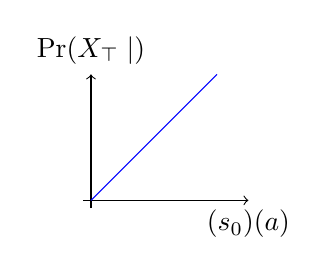
\begin{tikzpicture}[scale=2]
 \draw[->] (-0.05, 0) -- (1, 0) node[below]{$\sched(s_0)(a)$};
  	\draw[->] (0, -0.05) -- (0, 0.8) node[above] {$\Pr(X_{\lozenge\mathbf{\top}} \mid \sched)$};
  	%\draw[-,dashed] (0.4,0) -- (0.4,0.5184);
  	%\draw[-,dashed] (0.0,0.5184) -- (0.4,0.5184);
  \draw[ domain=0:0.8, smooth, variable=\x, blue] plot ({\x}, {\x});
\end{tikzpicture}
\caption{}
\end{subfigure}
\begin{subfigure}{0.38\columnwidth}
\centering
\begin{tikzpicture}[scale=2]	
 \draw[->] (-0.05, 0) -- (1, 0) node[below]{$\sched(s_0)(a)$};
  	\draw[->] (0, -0.05) -- (0, 0.8) node[above] {$H(\sched)$};
  	%\draw[-,dashed] (0.4,0) -- (0.4,0.5184);
  	%\draw[-,dashed] (0.0,0.5184) -- (0.4,0.5184);
 % \draw[ domain=0:1, smooth, variable=\x, blue] plot ({\x}, {15*(1-\x)*(1-\x)*(1-\x)*\x*\x});
\end{tikzpicture}
\caption{}
\end{subfigure}

\caption{Minimal ERCI problem.}
\end{figure}


\subsection{Preprocessing}
In this subsection, we preprocess the problem statement.
To ease the technical construction, without loss of generality, we make the following assumptions\footnote{We argue that these assumptions are indeed w.l.o.g.\ in Sec.~\ref{sec:assumptions}}: 
We assume the (graph structure underlying the) SG is acyclic, which we realise by means of unfolding the graph. 
Once we have the acyclic SG, we can also set the horizon $\horizon$ to be sufficiently long such that $\horizon$ is at least the length of the , and thus we drop any reference to $\horizon$ from here onwards.
As in \cite{DBLP:conf/cav/Vazquez-Chanlatte20}, we may represent this computation tree (typically) concisely using binary decision diagrams.
We calculate all states from which the $\pTwo$-player can enforce violating the hard constraint. We remove these states along with their in- and outgoing transitions. Any $\pOne$-policy now satisfies the hard constraint. 
We may now define a unique target state $\target$ and a unique sink state $\sink$ such that these are the only states without any outgoing transitions.  The set $X_{\lozenge\mathbf{\top}}$ denotes all paths with $\last{\path} = s_\top$.

\begin{mdframed}
\textbf{The Entropic Control Improvisation (ERCI) Problem}:
Given an acyclic SG $\sg$, including target states $s_\top$ and sink state $s_\bot$, thresholds $\scthreshold \in (0,1)$ and $\randomness \in [0,\infty)$,  find a $\pOne$-policy $\pOneSched \in \POneScheds$  such that for every $\pTwo$-policy $\pTwoSched \in \PTwoScheds$ \begin{compactenum}
	\item (\emph{soft constraint)} $\Pr(X_\varphi \mid \sched) \geq \scthreshold$
\item (\emph{randomness constraint}) $H(\sigma) \geq \randomness$
\end{compactenum}
where  $\sched = \langle \pOneSched, \pTwoSched \rangle$.
\end{mdframed}

\begin{example}
	
\end{example}



%%% Local Variables:
%%% mode: latex
%%% TeX-master: "main"
%%% End:
